\chapter{Simple Glaze Theory}
%-------------------------------------------------------------------------------
\section{Basic Chemistry}
Chemistry is the science which describes what substances are made of and how 
they combine with each other. This science uses special names and symbols which 
are described below.
%-------------------------------------------------------------------------------
\subsection{Elements and Compounds}
%-------------------------------------------------------------------------------
\subsubsection{Elements}
An element is made of only one kind of atom. It cannot be broken down into more 
simple substances. Oxygen (O) is the most common element on earth.
%-------------------------------------------------------------------------------
\subsubsection{Compounds}
A compound is composed of more than one element combined chemically. Water 
(H2O) is a compound made up of two atoms of hydrogen (H) and one atom of oxygen 
(O). Silica (SiO2) is another compound and consists of one atom of silicon (Si) 
and two atoms of oxygen (O). This is the most abundant material in the earth's 
crust. Two or more atoms combined form a molecule.
%-------------------------------------------------------------------------------
\begin{figure}[htbp!]
\centering
\begin{subfigure}{.45\textwidth}
\centering
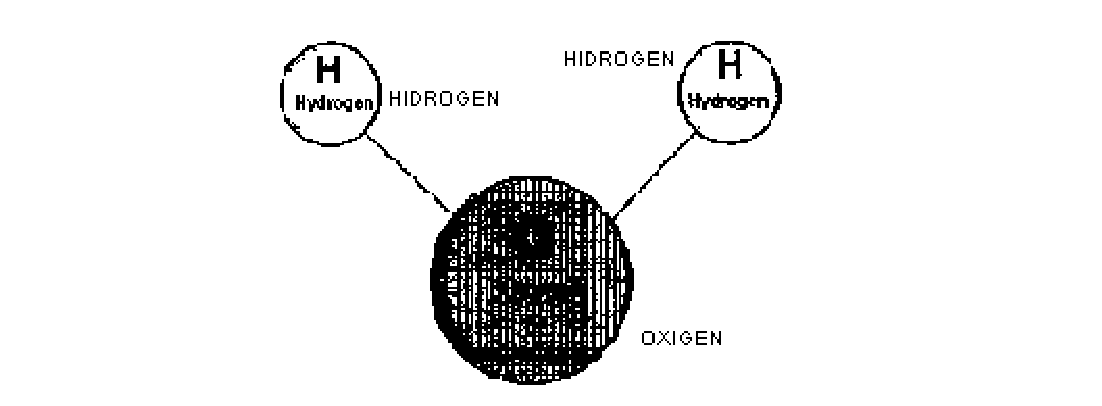
\includegraphics[width=1\linewidth]{img/molecule1.eps}
\caption{Water is two elements combined. A molecule of water consist of two 
atoms of hydrogen and one of oxygen.}
\label{fig:molecule1}
\end{subfigure}%
\hfill
\begin{subfigure}{.45\textwidth}
\centering
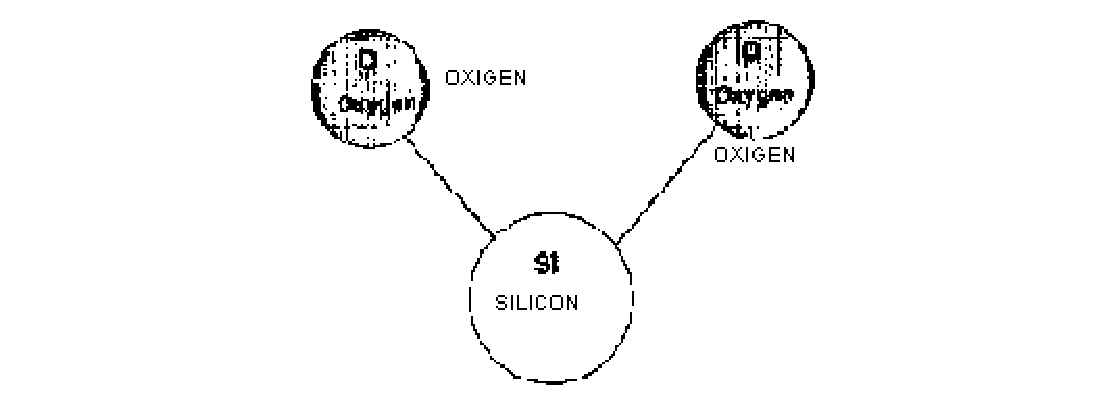
\includegraphics[width=1\linewidth]{img/molecule2.eps}
\caption{A molecule of the compound silica (sand) has two atoms of oxygen and 
one of silicon}
\label{fig:molecule2}
\end{subfigure}
\caption{Different molecules.}
\label{fig:molecules}
\end{figure}
%-------------------------------------------------------------------------------
Ceramic raw materials are usually in the form of oxides: an oxide is a compound 
that includes oxygen (O). Minerals are compounds.
%-------------------------------------------------------------------------------
\subsection{Solid, Liquid, Gas}
Solid, liquid and gas are the three states of matter. Most materials can exist 
in all of these states, depending on their temperature. A familiar example is 
water, which is solid below 0\degree C, liquid from 0\degree C to 100\degree C, 
and gas above 100\degree C.

Making glaze depends on mixing solids together, applying them on a pot and then 
changing them to liquid in the kiln. Some of the glaze materials also become 
gas during firing and leave the glaze. On cooling, the glaze again becomes 
solid.
%-------------------------------------------------------------------------------
\subsection{Mixture}
A mixture is a physical, not chemical, combination of compounds (and sometimes 
elements) and each compound remains chemically unchanged in the mixture. Air is 
a mixture of oxygen, carbon dioxide, nitrogen and other gases. A glaze made of 
feldspar, quartz and lime is prepared by combining the compounds as a mixture, 
but during firing a chemical combination takes place and the fired glaze 
becomes a compound.
%-------------------------------------------------------------------------------
\subsection{Chemical Symbols}
There are about 100 elements, and each of these has a name and a chemical 
symbol, which is used as an abbreviation of its name. Some of these symbols are 
the same as the first letters of the English name, but some are not!

For example:
%-------------------------------------------------------------------------------
\begin{itemize}
\item Oxygen is \ce{O}
\item Hydrogen is \ce{H}
\item Silicon is \ce{Si}
\item Alumina is \ce{Al}
\item Sodium is \ce{Na}
\item Lead is \ce{Pb}
\end{itemize}
%-------------------------------------------------------------------------------
Compounds are written in a similar way with capital letters marking the 
individual elements: for example, water \ce{H2O} and salt is \ce{NaCl}

The small number ``2'' in \ce{H2O} indicates that there are two atoms of 
hydrogen 
for each atom of oxygen in water. If there is no number, it is understood that 
there is only one atom -so salt is one atom of sodium and one atom of chlorine.

The formulas of complex ceramic materials are written as compounds of oxides 
with a raised period (·) between them to show they are chemically combined. For 
example potash feldspar is written:

\ce{K2O*Al2O3*6SiO2}

In the appendix the chemical formulas of other materials are listed.
%-------------------------------------------------------------------------------
\subsection{Chemical Reactions}
The formation of clay from feldspar can be written in chemical symbols:

\ce{K2O*Al2O3*6SiO2 + H2O -> Al2O3*2SiO2*2H2O + K2O + SiO2}

$Feldspar + Water \rightarrow Clay + Potash + Silica$

All materials are built up of elements which are chemically bonded together. 
When heated to a high temperature, chemical bonds can break down and the 
material will change its properties. The production of quicklime by heating 
limestone to 900\degree C is an example of this:

\ce{CaCO3 -> CaO + CO2}

$Limestone + Quicklime \rightarrow Carbon~Dioxide$

Carbon dioxide \ce{(CO2)} goes into the air, and the remaining quicklime 
\ce{(CaO)} is slaked with water and can then be mixed with sand to form mortar 
for house construction. The mortar sets when the calcium oxide \ce{(CaO)} takes 
back carbon dioxide \ce{(CO2)} from the air and thereby regains the hardness of 
the original limestone \ce{(CaCO3)}:


\ce{CaO + Co2 -> CaCO3}

$Soft~mortar + Air \rightarrow Set~mortar$
%-------------------------------------------------------------------------------
\subsection{Solutions and Suspensions}
%-------------------------------------------------------------------------------
\subsubsection{Solution}
A solution is a mixture of molecules. For example, sugar completely dissolves 
in water: the separate particles consist of molecules of sugar and water. Sugar 
and water remain a solution until the water evaporates.

The higher the temperature of the liquid, the more solid material can dissolve 
in the liquid. When no more solid can be dissolved the solution is called 
``saturated''.
%-------------------------------------------------------------------------------
\subsubsection{Suspension}
In a suspension the particles are bigger than molecules. A mixture of clay and 
water is a suspension. The clay particles are not changed by the water, and 
after some time the clay will settle at the bottom of the vessel. The clay is 
insoluble in water.
%-------------------------------------------------------------------------------
\subsection{Crystal Structures}
If we heat water to 90\degree C and add salt \ce{(NaCl)}, it will become 
dissolved in the water. If we continue to add salt until no more salt can be 
dissolved, the suspension is saturated with salt. If we let the solution cool 
to room temperature (20\degree C) the water can hold much less salt in 
solution, with the result that some of the salt will separate in the form of 
salt crystals.

All minerals have the form of crystals. When the water cools, the excess salt 
molecules start to combine with one another in regular patterns like small 
building blocks. The way the salt molecules connect to one another is very 
orderly and produces a cube-shaped crystal. Different materials will produce 
crystals of different shapes. The shape of a mineral's crystal is used to 
identify it.
%-------------------------------------------------------------------------------
\begin{figure}[htbp!]
\centering
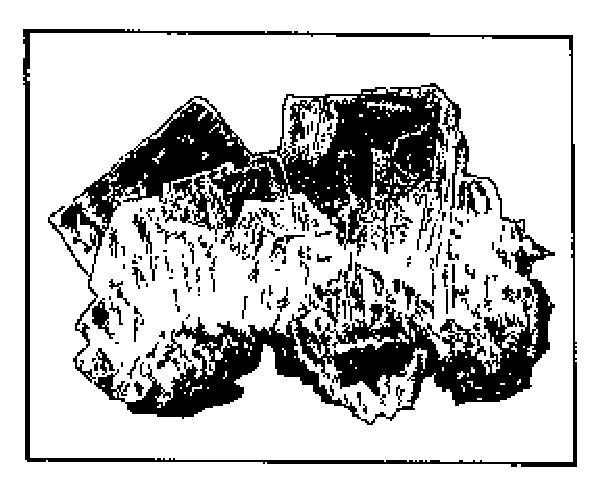
\includegraphics[width=0.5\linewidth]{img/salt.eps}
\caption{The cubic shape of a salt crystal.}
\label{fig:salt}
\end{figure}
%-------------------------------------------------------------------------------
\section{Glaze Structure}
Glaze is similar to glass. Making glazes is confusing because there are so many 
raw materials that can be used. However, all of these raw materials can be 
broken down into three categories:
%-------------------------------------------------------------------------------
\begin{itemize}
\item Flux
\item Glass former
\item Stabilizer
\end{itemize}
%-------------------------------------------------------------------------------
All glazes require these three components. The main glass former is silica, the 
main stabilizer is kaolin, and the rest of the glaze is composed of one or more 
fluxes.
%-------------------------------------------------------------------------------
\subsection{Glass Structure}
Silica \ce{(SiO2)} alone will make an excellent glaze if it is fired to its 
melting point (1715\degree C). Since this temperature is too high for ordinary 
kilns, other materials are added to lower the melting point of silica. Quartz 
is a crystalline form of silica found in nature. If a glaze forms quartz 
crystals when it cools, it will not be transparent, since light is refracted in 
many different directions by the crystal faces. Because glass or glaze is not 
usually crystalline, this does not happen.

A glaze or glass is a mixture of compounds that melts when heated. The melted 
liquid glass is like a solution. When the liquid cools, crystals start to form 
in a similar way as in a salt solution. However, the liquid glaze is very 
viscous (meaning sticky and semifluid) and the molecules cannot easily move 
around to form a regular crystalline pattern. So normally no crystals form 
during cooling, and the glaze remains clear like a liquid.

Glaze is, therefore, like a solid solution and is sometimes called a 
supercooled liquid.
%-------------------------------------------------------------------------------
\subsection{Fluxes}
Fluxes are the materials which lower the melting point of a glaze. They can be 
called melters.

Silica melts by itself but at a very high temperature. Therefore it needs 
additions of flux to make a practical glaze. The most common flux for 
temperatures below 1100\degree C is lead oxide \ce{(PbO)}, but since it is 
poisonous it is no longer used in modern crockery glazes. Another powerful flux 
is boron or boric oxide, \ce{B2O3}, which is not poisonous and is used in 
glazes in 
the form of borax or boric acid. There are many other fluxes which contribute 
various properties of hardness, opacity, color response etc.

Fluxes are also called basic oxides or network modifiers.
%-------------------------------------------------------------------------------
\subsection{Glass Formers}
Silica forms the main part of all glazes and is called a glass-former. The 
other glass-former is boron. Silica and boron are the building blocks of a 
glass or glaze. Other materials are only used to modify their behavior in the 
glaze.

Titanium oxide \ce{(TiO2)}, tin oxide \ce{(SnO2)} and zirconium oxide 
\ce{(ZrO2)} also belong to this group. Sometimes they are called the acidic 
oxides or network former, or the acid portion of the glaze.
%-------------------------------------------------------------------------------
\subsection{Stabilizers}
Aluminum oxide, \ce{Al2O3}, is added to make the melted glaze stiffer, so that 
it will not run off the pots during firing. It is called a stabilizer. Other 
words for stabilizer are: amphoteric, neutral or intermediate oxide.

Aluminum oxide has a high melting point and will increase the melting point of 
the glaze. It is usually added to the glaze as kaolin (china clay).

(Boron is termed a stabilizer in the USA but a glass former in Europe.)
%-------------------------------------------------------------------------------
\section{Effect of Heat}
As heat is increased, the molecules in the glaze move faster, resulting in 
drying, sintering, melting and gas escape. All of these effects occur when the 
glaze molecules move so fast that they start to break down, releasing some of 
their atoms and combining with other molecules to form the glaze.
%-------------------------------------------------------------------------------
\subsection{Drying}
When the powdered glaze on the surface of the ceramic ware is heated, the water 
evaporates above 100\degree C (no matter how dry the glaze seems to be, there 
will 
always be some water remaining in it). The glaze layer should be as dry as 
possible before setting in the kiln. If the glaze layer dries too fast when 
firing starts, it may crack. This can cause crawling of the glaze after it 
melts.
%-------------------------------------------------------------------------------
\subsection{Sintering, Melting, Gas Escape}
%-------------------------------------------------------------------------------
\subsubsection{Sintering}
As the temperature rises above 600\degree C, the sintering of the glaze powder 
starts. 
Sintering also takes place in the clay at this temperature. Sintering means 
that the glaze (or clay) particles start to stick to one another where they 
touch. The finer the glaze particles are ground, the earlier the sintering will 
start and the stronger the bond will become.
%-------------------------------------------------------------------------------
\begin{figure}[htbp!]
  \centering
  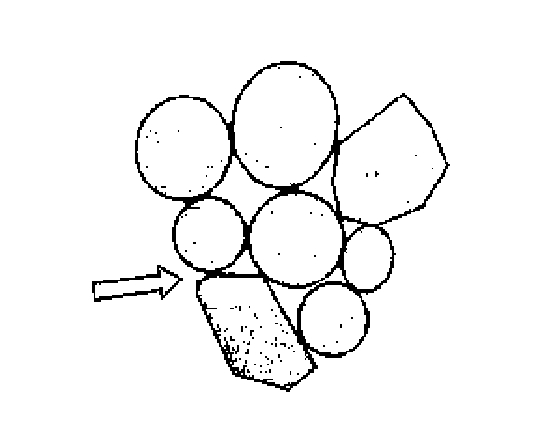
\includegraphics[width=0.5\linewidth]{img/sintering.eps}
  \caption{The glaze particles are enraged many thousand times showing 
  sintering in a glaze heated to 600\degree C. At the points of contact (arrow) 
  a weak 
  bond is formed.}
  \label{fig:sintering}
\end{figure}
%-------------------------------------------------------------------------------
\subsubsection{Fusion}
As the temperature rises further, the most fusible (easy melting) materials in 
the glaze start to melt. This is celled fusion. The refractory (hard melting) 
particles are surrounded by the liquid materials and are slowly included in the 
liquid.

The temperature at which melting starts depends on the materials in the glaze. 
Silica alone melts at 1715\degree C, but with additions of other materials the 
melting point will go down. Aluminum oxide \ce{(Al2O3)} melts at 2050\degree C 
and calcium oxide \ce{(CaO)} at 2570\degree C, but a mixture of 62\% 
silica, 14.75\% aluminum oxide and 23.25\% lime melts at only 1170\degree 
C. A mixture which has a lower melting point than any of the single materials 
in the mixture is called an eutectic.

A mixture with many different materials will form eutectics (and will melt) at 
a lower temperature. Fine grinding of the glaze materials and prolonged firing 
time above the sintering temperature will also lower the melting point.

When fusion starts, the compounds also start to change. The chemically bonded 
water in clay has already been released. Around 900\degree C, limestone 
\ce{(CaCO3)} releases carbon dioxide \ce{(CO2)} and so do other materials 
containing carbonates, like barium carbonate \ce{(BaCO3)}. Gases of sulfates, 
oxides etc. are also released both from the glaze and from the body. These 
gases have to pass through the glaze layer. This action mixes the glaze, 
helping it to become homogeneous.

In the beginning the melted glaze is very stiff (high viscosity), but as the 
temperature keeps rising the glaze becomes more fluid and, when watching the 
melting glaze surface through a spyhole in the kiln, bubbling or even boiling 
can be seen. When the glaze reaches its maturing temperature, the reactions 
stop and the glaze becomes smooth.
%-------------------------------------------------------------------------------
\begin{figure}[htbp!]
\centering
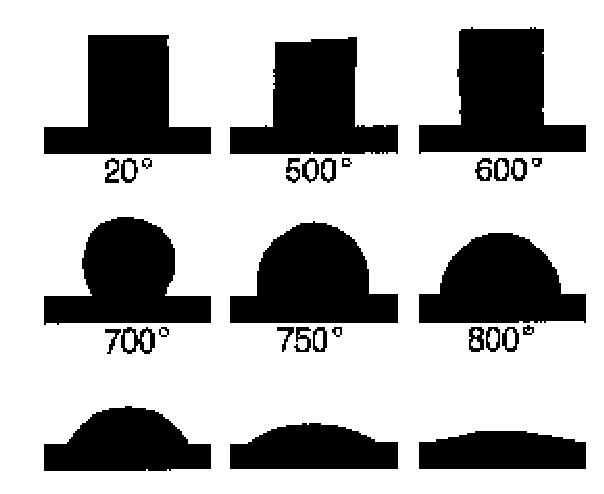
\includegraphics[width=0.5\linewidth]{img/fusion.eps}
\caption{A cube of glaze is gradually heated up to 1000\degree C. At 500\degree 
C the glaze shrinks slightly (sintering), but at 600\degree C it swells as 
gases develop. Melting starts before 700\degree C and is completed at 
1000\degree C.}
\label{fig:fusion}
\end{figure}
%-------------------------------------------------------------------------------
\subsection{Materials Which Increase or Decrease Melting Point}
\label{sec:meltingpointsec}
Table~\ref{tab:glazephysicalcharacteristics} shows the oxides according to 
their influence on 
melting temperature.
%------------------------------------------------------------------------------
\begin{center}
        \renewcommand{\arraystretch}{1.5}
        \begin{table}\centering
\begin{tabular}{|c|c|c|c|c|c|}\hline
    \multicolumn{2}{|c}{\textbf{Melting Point}}
    &\multicolumn{2}{|c|}{\textbf{Viscosity}}
    &\multicolumn{2}{c|}{\textbf{Surface Tension}}
\\\hline\hline
%------------------------------------------------------------------------------
\textbf{Oxide}&\textbf{Effect}&\textbf{Oxide}&\textbf{Effect}&\textbf{Oxide}
&\textbf{Effect}\\\hline\hline
%------------------------------------------------------------------------------
\ce{Al2O3}&Raise&\ce{Al2O3}&Increase&\ce{Al2O3}&Increase\\\hline
%------------------------------------------------------------------------------
\ce{SiO2}&-&\ce{ZrO2}&-&\ce{ZrO2}&-\\\hline
%------------------------------------------------------------------------------
\ce{MgO}&-&\ce{SiO2}&-&\ce{ZnO}&-\\\hline
%------------------------------------------------------------------------------
\ce{Cr2O3}&-&\ce{Cr2O3}&-&\ce{CaO}&-\\\hline
%------------------------------------------------------------------------------
\ce{SnO2}&-&\ce{NiO}&-&\ce{SnO2}&-\\\hline
%------------------------------------------------------------------------------
\ce{ZrO2}&-&\ce{Fe2O3}&-&\ce{Cr2O3}&-\\\hline
%------------------------------------------------------------------------------
\ce{NiO}&-&\ce{TiO2}&-&\ce{NiO}&-\\\hline
%------------------------------------------------------------------------------
\ce{Fe2O3}&-&\ce{CaO}&-&\ce{BaO}&-\\\hline
%------------------------------------------------------------------------------
\ce{TiO2}&-&\ce{MgO}&-& \ce{SrO}&-\\\hline
%------------------------------------------------------------------------------
\ce{CaO}&-&\ce{ZnO}&-&\ce{Fe2O3}&-\\\hline
%------------------------------------------------------------------------------
\ce{ZnO}&-&\ce{SrO}&-&\ce{SiO2}&-\\\hline
%------------------------------------------------------------------------------
\ce{BaO}&-&\ce{BaO}&-&\ce{TiO2}&-\\\hline
%------------------------------------------------------------------------------
\ce{FeO}&-&\ce{CoO}&-&\ce{Li2O}&-\\\hline
%------------------------------------------------------------------------------
\ce{CoO}&-&\ce{MnO}&-&\ce{Na2O}&-\\\hline
%------------------------------------------------------------------------------
\ce{CuO}&-&\ce{PbO}&-&\ce{K2O}&-\\\hline
%------------------------------------------------------------------------------
\ce{MnO}&-&\ce{K2O}&-&\ce{B2O3}&-\\\hline
%------------------------------------------------------------------------------
\ce{PbO}&-&\ce{Na2O}&-&\ce{PbO}&Decrease\\\hline
%------------------------------------------------------------------------------
\ce{B2O}3&-&\ce{B2O3}&-&&\\\hline
%------------------------------------------------------------------------------
\ce{Na2O}&-&\ce{Li2O}&Decrease&&\\\hline
%------------------------------------------------------------------------------
\ce{K2O}&-&&&&\\\hline
%------------------------------------------------------------------------------
\ce{Li2O}&Lower&&&&\\\hline
%------------------------------------------------------------------------------
\end{tabular}
\caption{Materials which affect physical characteristics of a 
glaze. Note this scale is not linear and depends on variables like firing 
temperature, amount of oxide in the glaze, and (for surface tension) the glaze 
viscosity.}
\label{tab:glazephysicalcharacteristics}
\end{table}
\end{center}
%------------------------------------------------------------------------------
\section{Melted Glaze Behavior}
\subsection{Fluid State}
The fluid state of the glaze should be maintained long enough to allow all 
bubbles time to escape, so the glaze layer can heal over the holes left by the 
escaping bubbles. If a glaze tends to produce pinholes and craters, it can be 
given a soaking period (keeping the kiln at maturing temperature for some time) 
or the firing temperature can be raised in order to make the glaze more fluid 
(reduce viscosity).

If the glaze is too fluid, it will run off the pot or the fluid glaze will soak 
into a porous body leaving matt, dry spots on the surface.

Table~\ref{tab:glazephysicalcharacteristics} shows materials which increase or 
decrease viscosity:
%------------------------------------------------------------------------------
\subsection{Surface Tensions}
\label{sec:surfacetension}
To understand surface tension, fill a glass with water to the rim and look at 
the water surface. The middle of the water surface will be higher than the rim, 
but the water will not run over. The surface tension of the water holds it as 
if it were held by a plastic membrane.

A small amount of water forms a spherical drop. Larger amounts of water flatten 
the spherical form because the force of gravity increases with the weight of 
water. The fluid glaze behaves in a similar manner, and if the surface tension 
of the fluid glaze is too high the glaze will pull itself into small islands, 
leaving the clay body uncovered. This is called crawling.

Different oxides have different effects on glaze surface tension, as 
table~\ref{tab:glazephysicalcharacteristics} illustrates.

Increasing temperature lowers the surface tension as 
figure~\ref{fig:fusion} illustrates. At 800\degree C the glaze forms a half 
globe but at 1000\degree C it has completely flattened out.
%-------------------------------------------------------------------------------
\begin{figure}[htbp!]
  \centering
  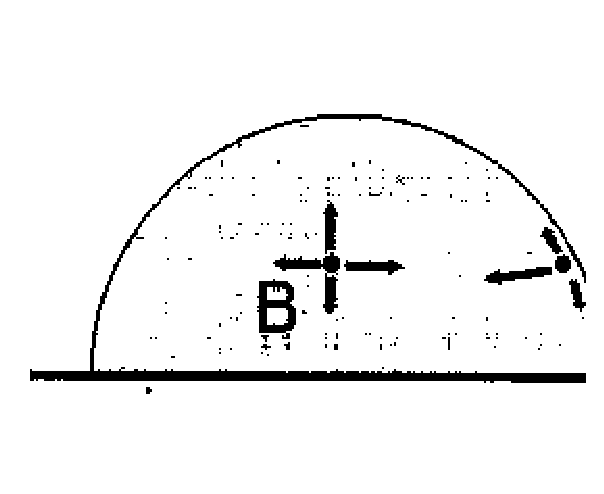
\includegraphics[width=0.5\linewidth]{img/surfacetension.eps}
  \caption{Surface tension is created by the difference of forces acting on 
  water 
    in the center (B) and at the surface (A). A water particle at B has forces 
    of traction of the water around it evenly distributed. But at A the force 
    is 
    mainly directed away from the surface. This difference causes water to form 
    itself ion spherical drops.}
  \label{fig:surfacetensionimage}
\end{figure}
%------------------------------------------------------------------------------
\subsection{Crawling}
Crawling is caused by two factors:
%------------------------------------------------------------------------------
\begin{itemize}
\item high surface tension of the glaze
\item difficulty for the glaze to stick to the body
\end{itemize}
%------------------------------------------------------------------------------
If the body surface is greasy or dusty the problem is aggravated. Crawling may 
also happen if the glaze layer cracks before it is sintered. This happens if 
the glaze contains a high amount of clay or has been ground for too long in the 
ball mill. The surface tension will then pull the glaze away from the cracks.
%-------------------------------------------------------------------------------
\begin{figure}[htbp!]
  \centering
  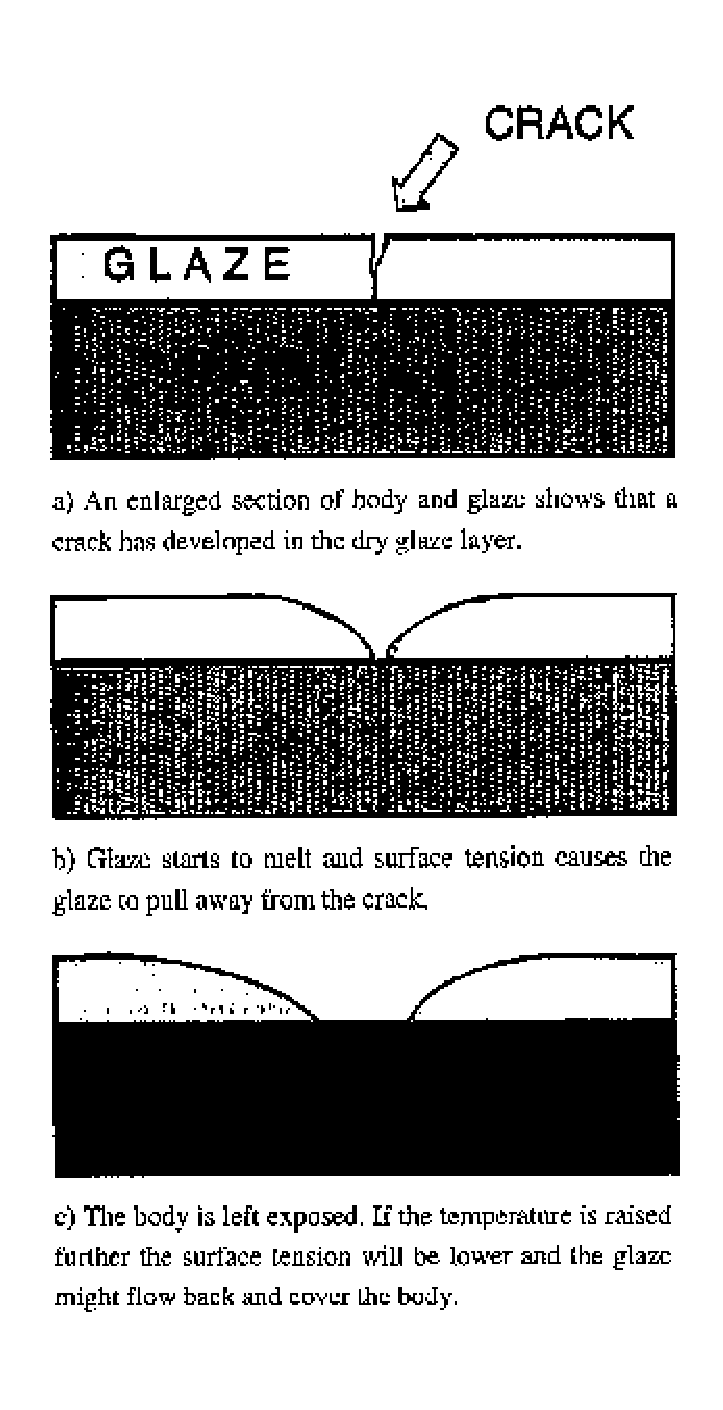
\includegraphics[width=0.5\linewidth]{img/crawling.eps}
  \caption{Crawling.}
  \label{fig:crawling}
\end{figure}
%-------------------------------------------------------------------------------
\subsection{Craters and Pinholes}
The lower the surface tension, the shinier the surface of the glaze becomes and 
the easier it is for the glaze to heal over craters, bubbles and pinholes.

Interesting effects can be obtained by applying glazes with different surface 
tensions on top of each other.

Surface tension, viscosity and melting temperature are interrelated, so when 
replacing materials all three will be affected.
%-------------------------------------------------------------------------------
\section{Interface between Glaze and Body}
During firing the glaze interacts with the clay body. Some of the glaze will 
sink into the body and some of the body material will mix with the glaze so 
that an intermediate layer is formed between the body and the glaze. This layer 
bonds the clay and glaze together. It is called the glaze/body interface or 
``buffer'' layer.
%-------------------------------------------------------------------------------
\subsection{Effects of Interface}
Some of the coloring oxides in the body may enter the glaze and change its 
colon The higher the firing temperature the stronger the interface layer. The 
interface layer produces a strong bond between glaze and body that reduces the 
tendency to craze or peel.

Glazing on greenware (raw glazing or green glazing or single firing) promotes 
interaction between body and glaze. If too much of the glaze's flux combines 
with the refractory materials in the body, the glaze may become matt or dry.
%-------------------------------------------------------------------------------
\begin{figure}[htbp!]
  \centering
  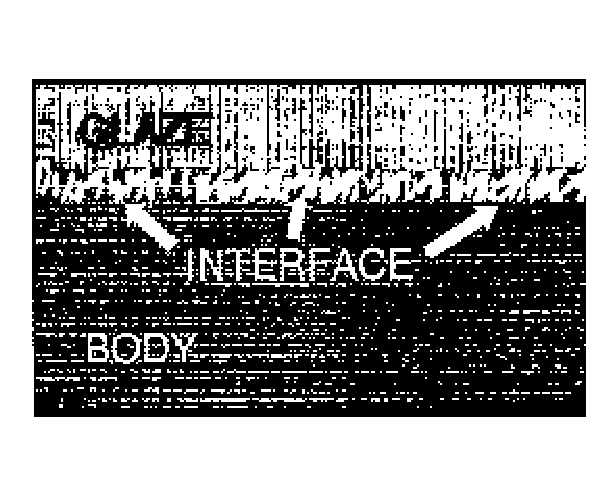
\includegraphics[width=0.8\linewidth]{img/interface.eps}
  \caption{Interface layer created during firing by mixing of materials in the 
  body and the glaze.}
  \label{fig:interface}
\end{figure}
%-------------------------------------------------------------------------------
\section{Cooling and Crystal Formation}
Glaze or glass is called a supercooled liquid because, during cooling, crystals 
have no time to form in the rather sticky mass, and glass by definition does 
not contain crystals. But some matt glazes and opaque glazes depend on the 
formation of crystals. For these, cooling should be slow to allow the crystals 
to grow. \ce{ZnO}, \ce{BaO}, and \ce{TiO2} are used for making matt glazes, but 
if cooling is rapid the glaze will become glossy instead of matt.

To avoid crystal formation, glossy transparent glazes should be cooled quickly 
after the maturing temperature has been reached.
%-------------------------------------------------------------------------------
\section{Transparency and Opacity}
Transparency is the property of allowing light to pass through the glaze to-the 
clay below. Transparent glazes may be colorless or have color in them - 
transparent blue, green, brown etc. It is necessary to use transparent glazes 
in combination with underglaze decoration. Transparent glazes are always shiny.

Opacity is the property of not allowing light to pass through the glaze. 
Colorless opaque glazes usually look white or gray. When coloring oxides are 
added, they can be any possible colors. They generally are used with overglaze 
or on-glaze.

It is possible to make glazes with every degree of transparency or opacity, 
such as semitransparent or semiopaque.
%-------------------------------------------------------------------------------
\begin{figure}[htbp!]
  \centering
  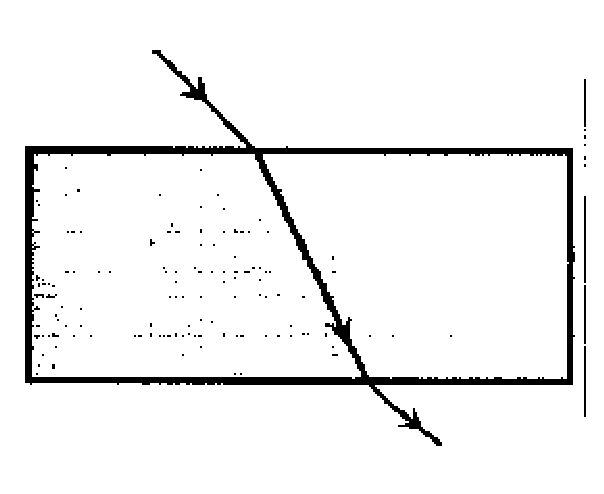
\includegraphics[width=0.5\linewidth]{img/transparency.eps}
  \caption{Section of a window glass. A beam of light passes through it - it is 
  transparent. The lights dissection is slightly bent when passing from one 
  medium (air) to another (glass). This is called refraction.}
  \label{fig:transparency}
\end{figure}
%-------------------------------------------------------------------------------
\subsection{Refraction of Light}
Transparency and opacity are determined by the glaze's ability to transmit 
light. When light strikes a transparent glaze, most of it passes through the 
glaze layer to the clay underneath, and the color we see is determined by the 
color of the clay. Thus, a transparent glaze on a brown clay body will look 
brown whereas the same glaze on a white clay body will look white. If the 
transparent glaze is colored, the clay body color will be changed by the fact 
that the glaze is green or blue, etc.
%-------------------------------------------------------------------------------
\begin{figure}[htbp!]
  \centering
  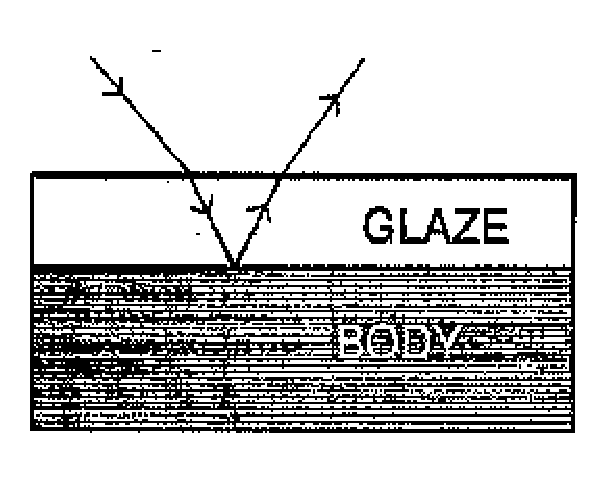
\includegraphics[width=0.5\linewidth]{img/reflecting.eps}
  \caption{A transparent glaze reflects the color of the underlying body.}
  \label{fig:reflecting}
\end{figure}
%-------------------------------------------------------------------------------
Opaque glazes have a large number of particles in them that reflect light, 
without allowing it to pass through the glaze. So we are not able to see 
through the glaze. Thus what we observe is only the surface of the glaze, which 
is not affected by the color of the clay underneath.

Semitransparent glazes have smaller numbers of light-reflecting particles, so 
they look cloudy or milky, and their color will be affected by the clay color 
underneath.

Transparent glazes can be made opaque by the addition of opacifiers, which are 
finely ground particles that do not enter into the melting of the glaze. These 
particles stay suspended in the glaze and reflect light. This is similar to 
mixing clay with water, which makes the water opaque.

Opaque glazes cannot be made transparent without changing their formula (unless 
they are transparent glazes with opacifier added).

The causes of opacity in glazes can be divided into 4 groups:
%-------------------------------------------------------------------------------
\begin{enumerate}
\item Presence of very fine particles, which do not dissolve in the glaze melt. 
The light going through the glaze is scattered by the fine particles. Tin oxide 
\ce{(SnO2)} and zircon \ce{(ZrSiO4)} are used for this.
\item Crystals formed in the glaze during cooling will scatter the light, 
causing opacity. Titanium dioxide \ce{(TiO2)} recrystallizes if the cooling is 
slow and can make glazes opaque.
\item Opacity is also caused when two melting phases of the glaze do not mix. 
The light will be scattered when it passes through the border between the two 
different melts. This takes place in boron glazes and with calcium phosphate 
(bone ash).
\item Gas bubbles scatter the light and produce opacity. This type of opacity 
is difficult to control and the method is not recommended.
\end{enumerate}
%-------------------------------------------------------------------------------
In practice, a combination of the four methods is used. For example, an opaque 
glaze can be made with boron and additions of lime, zinc oxide and zircon.
%-------------------------------------------------------------------------------
\subsection{Materials Causing Opacity}
The best opacifier is tin oxide, which will make most glazes opaque in 
additions of up to 7\%. However, it is a very expensive material and today is 
only used for special high-cost products.

Commercially available opacifiers are based on zirconium silicate, prepared 
with other additions such as magnesia and zinc oxide. They are marketed under 
names such as ``zirconium opacifier'', ``zirconium silicate'', ``zinc zirconium 
silicate'' and ``magnesium zirconium silicate''. Most of these are added to 
glazes 
from 5 to 10\% and produce different results depending on the type of base 
glaze. They also vary widely in quality, and it is important to test them 
before ordering a large quantity. Zirconium opacifiers have the disadvantage of 
making glazes more refractory and often cause pinholing problems.

The main opacifiers are:
%-------------------------------------------------------------------------------
\begin{itemize}
\item Tin oxide, \ce{SnO2}
\item Zircon, zirconium silicate, \ce{ZrSiO4}
\item Titanium dioxide, \ce{TiO2}
\item Alumina, \ce{Al2O3} (high content in boron glazes will reduce opacity)
\item Calcium oxide, \ce{CaO} (improves opacity in boron glazes)
\item Zinc oxide, \ce{ZnO}
\item Calcium phosphate, bone ash, \ce{Ca3(PO4)2}
\end{itemize}
%-------------------------------------------------------------------------------
\subsection{Particle Size}
The finer the particle size of the opacifier, the better it works. Zircon is 
often included in the frit batch for greater opacity. In this way opacity is 
obtained with less zircon, thus reducing some of zircon's bad side effects like 
high viscosity and the tendency to cause pinholes. Unfortunately the addition 
of zircon to the frit increases its melting point, making it more difficult to 
run it off the frit kiln. It also increases the hardness of the frit so much 
that it may be difficult to grind it with ordinary pebbles and ball mill lining.

It is important to make sure that the opacifier is well dispersed in the glaze. 
The fine particles tend to lump together. This reduces the opacity effect. By 
ball milling the opacifier together with the glaze a good dispersion is assured.
%-------------------------------------------------------------------------------
\section{Shiny or Matt Glaze}
Glazes are also defined by the way they reflect light: they may be shiny or 
matt or in between.
%-------------------------------------------------------------------------------
\subsubsection{Shiny Glaze}
Shiny glazes are also known as ``glossy'' or ``bright''. They have the property 
of 
reflecting light like a mirror. They are best for utilitarian wares, sanitary 
ware and insulators, as they are easy to wash and do not scratch easily.
%-------------------------------------------------------------------------------
\begin{figure}[htbp!]
  \centering
  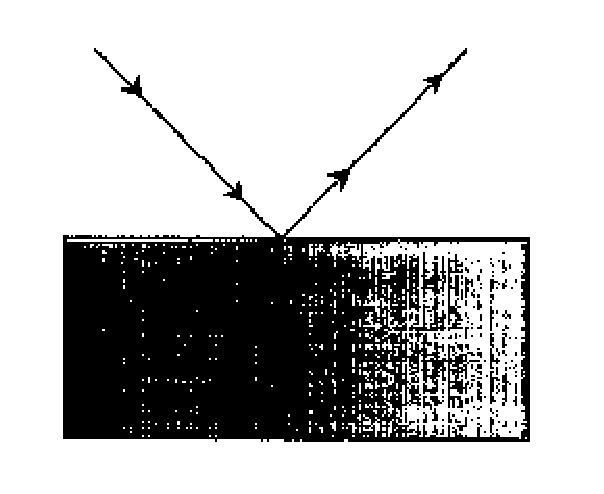
\includegraphics[width=0.5\linewidth]{img/glossyglaze.eps}
  \caption{A glossy glaze with a smooth surface reflects the light without 
  scattering it.}
  \label{fig:glossyglaze}
\end{figure}
%-------------------------------------------------------------------------------
\subsubsection{Matt Glaze}
Matt glazes are also known as ``dull'' or ``non-reflective''. Their surface can 
vary from smooth to very rough. They are useful for decorative wares and are 
very popular for floor tiles, which need to be beautiful but not slippery. The 
matt surface is not functional for dinnerware, because used with cutlery it 
makes an unpleasant sound and scratches easily.
%-------------------------------------------------------------------------------
\subsection{Materials Causing Mattness}
%-------------------------------------------------------------------------------
\subsubsection{Underfiring}
As glaze begins to melt, it becomes glassy. If the firing is stopped before the 
glaze is completely melted, even glossy glazes will appear matt. Often these 
underfired glazes will have other problems such as blisters and pinholes, but 
some glossy glazes make very good matt glazes if fired a few cones below their 
normal temperature. Similarly, adding refractory oxides to a glaze (such as 
china clay or calcium carbonate) will produce a matt glaze that really is just 
an underfired glossy glaze.
%-------------------------------------------------------------------------------
\subsubsection{Crystalline Matt}
Crystalline matt glazes develop small crystals which break up light (see 
Figure~\ref{fig:crystallinematt}). This type of matt glaze usually produces a 
more smooth surface than underfired matt glazes. Some matt glazes depend on 
slow cooling to have time for the crystals to develop.

Barium carbonate, zinc oxide, titanium dioxide, magnesium oxide and calcium 
oxide are the agents for crystal matt glazes.
%-------------------------------------------------------------------------------
\begin{figure}[htbp!]
  \centering
  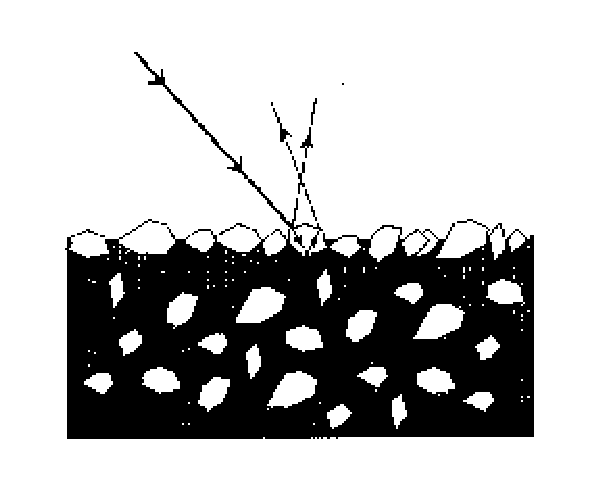
\includegraphics[width=0.5\linewidth]{img/crystallinematt.eps}
  \caption{Surface of crystal matt glaze enlarged several hundred times. 
    Crystals in the glaze scater the light by sending it in many different 
    directions.}
  \label{fig:crystallinematt}
\end{figure}
%-------------------------------------------------------------------------------%-------------------------------------------------------------------------------
\subsection{Other Causes}
Sometimes glazes that should be glossy will become matt. Some reasons 
are:
\begin{itemize}
\item Some of the flux materials may evaporate during firing.
\item Sulfates from fuel may settle on the surface of the glaze.
\item The glaze is applied too thin.
\item The glaze was not mixed sufficiently or not sieved finely enough.
\end{itemize}
%-------------------------------------------------------------------------------